\section{Computation as the graph grows}
\label{sec:computation}
Native timing logs separate the local solver update, the complete nonterminal timer callback, and peer-belief service responses. The analysis joins timing and statistics by robot and iteration, validates new-factor/value counts, and checks cumulative owned nodes against admitted graph prefixes. It retains 842 timed updates and 3,930 service requests. One terminal timer callback per robot is not recorded by the native CSV and is never filled with zero.
\begin{table}[htbp]
\centering\small
\caption{Native elapsed wall-time measurements. All duration columns are in milliseconds.}
\label{tab:timing}
\begin{tabular}{lrrrr}
\toprule
Timed region & Samples & Median (ms) & P95 (ms) & Maximum (ms) \\
\midrule
Local solver update & 842 & 0.351 & 1.003 & 4.499 \\
Full nonterminal callback & 842 & 1.629 & 32.230 & 1188.685 \\
Peer-belief service & 3,930 & 0.379 & 2.385 & 190.248 \\
\bottomrule
\end{tabular}
\par\vspace{5pt}\begin{minipage}{0.97\linewidth}\footnotesize The full callback contains the local solver update, so rows must not be added. Peer services run separately. Fourteen terminal callbacks, final geometry validation and pre-update early returns are outside the timing coverage.\end{minipage}
\end{table}


The solver call takes 0.351\,ms median and 4.499\,ms maximum. Its timer excludes input and geometry preparation. The broader callback takes 1.629\,ms median, 32.230\,ms at the 95th percentile, and 1.189\,s maximum, including the startup/admission spikes in Fig.~\ref{fig:timing-progress}. It includes lock waiting, successful input preparation, registration preparation, solver update, residual/statistics computation and asynchronous request submission. Calls returning before an update, separate PCM/geometry-exchange callbacks, and Python bridge work are outside this timer.

Peer-service timings separately include lock waiting, cavity marginalization and response packing. Their median is 0.379\,ms and maximum is 190.248\,ms. Services do not carry wall timestamps: plotting assigns each to its serving robot's iteration timestamp, with approximate temporal location. Five requests preceding iteration one appear only in the retained data and duration summary. Update plot timestamps are the corresponding statistics-receipt times. All durations are elapsed wall time from native timers, not CPU time or synchronized GPU kernel measurements.

\begin{figure}[p]
\centering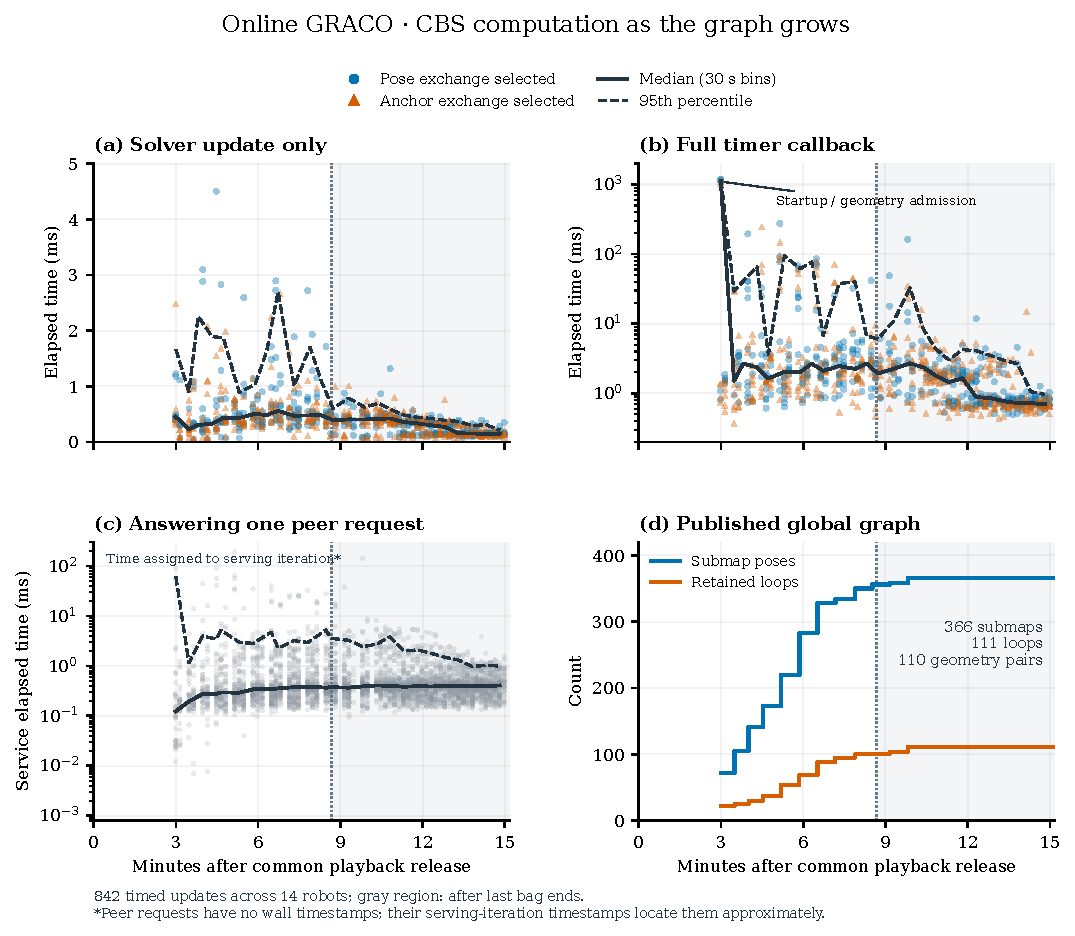
\includegraphics[width=\linewidth]{../output/pdf/cbs-update-progress.pdf}
\caption{CBS computation throughout the online experiment. Points are recorded local updates or service responses; solid and dashed curves show median and 95th percentile within 30\,s bins. Pose/anchor colors identify the randomly selected outgoing exchange after an update, not two separate solver kernels. The gray region follows the last bag's end. The graph grows to 366 submap poses and 111 retained loops, including 110 geometry pairs. Peer-service times are positioned approximately by serving iteration. No missing terminal timer values are imputed.}
\label{fig:timing-progress}
\end{figure}

The global graph is distributed across 14 optimizers: the largest recorded local estimate has 61 variables, including owned submaps, peer separator poses and anchors. Figure~\ref{fig:local-scaling} therefore relates cost to local variable count as well as global progress. No sharp update-cost increase appears within this tested range. The late reduction in cost coincides with fewer new factors and beliefs and a fixed graph; it does not show that larger graphs are intrinsically cheaper. One concurrent run with caching and varying geometry cannot establish an asymptotic complexity bound.

\begin{figure}[htbp]
\centering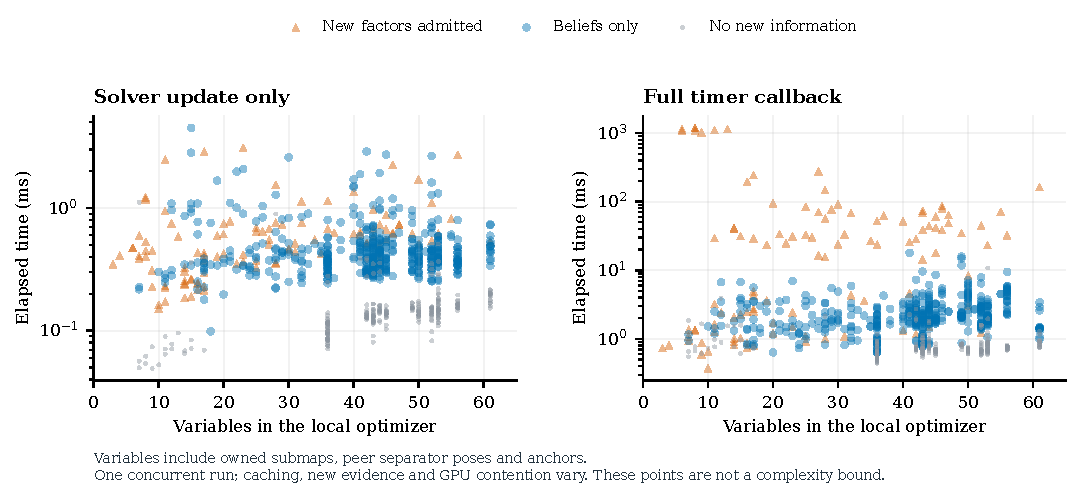
\includegraphics[width=\linewidth]{../output/pdf/cbs-local-graph-scaling.pdf}
\caption{Measured local computation versus optimizer variable count. New-factor admission has a distinct preparation cost, visible in full callbacks. Belief-only and no-new-information updates remain inexpensive over the observed range. Counts are local, not the global 366-node graph size; geometry budgets, graph structure and concurrent GPU load are not held constant.}
\label{fig:local-scaling}
\end{figure}

Short local computation is distinct from complete online latency. Asynchronous peer responses, prefix readiness, common-reference propagation and the configured settling schedule can delay publication while individual updates are inexpensive. The 10\,s update request does not promise a settled result every 10\,s. Final geometry validation, executed on the unlogged terminal path, is outside the reported timer maxima.

The full simultaneous pipeline, including odometry, preparation, recording and distributed processing, takes 913.15\,s wall time and 6,617.64 process-tree CPU seconds. Peak simultaneous process-tree RSS is 42.34\,GiB; shared pages may be counted multiple times. Whole-device GPU allocation peaks at 4,135\,MiB and includes device/driver overhead and any unrelated activity. These are all-14 workstation measurements, not per-robot memory requirements or Jetson Orin NX validation.
\FloatBarrier
